\documentclass[hyperref={pdfpagelabels=false}]{beamer}
% [hyperref={pdfpagelabels=false}] prevent from warning
% [notes] Notizen mit ausgeben
% [notes=only] nur Notizen ausgeben
% [handout] Overlays ignorieren

\usepackage{eurosym} % Eurozeichen: \euro
%\usepackage{subfigure} % Geteilte Abbildungen (subfig geht nicht bei beamer)
%\usepackage[german]{babel} % Unterst�tzung der deutschen Sprache
\usepackage[latin1]{inputenc} % Umlaute k�nnen direkt eingegeben werden
%\usepackage{graphicx} % Einbindung von Graphiken
\usepackage{booktabs} % toprule, midrule, bottomrule
\usepackage{calc} % Berechnungen von H�hen und Breiten
%\usepackage{animate}

% choose one of the following to prevent from font warnings
  %\let\Tiny=\tiny
  \usepackage{lmodern}
% print notes on the same page
  %\usepackage{pgfpages}
  %\setbeameroption{show notes on second screen=right}

% %%%%%%%%%%%%%%%%%%%%%%%%%%%%%%%%%%%%%%%%%%%%%%%%%%%%%%%%%%%%%%%%%%%%%%%%% %
% Ausgelagerte Makros und Stile                                             %
% %%%%%%%%%%%%%%%%%%%%%%%%%%%%%%%%%%%%%%%%%%%%%%%%%%%%%%%%%%%%%%%%%%%%%%%%% %

% Einstellung von Standardthemes
%\usepackage{beamerthemesplit}
%\usepackage{beamerthemeshadow}
\useinnertheme{default}
% default, circles, rectangels, rounded, inmargin
\useoutertheme{default}
% default, infolines, miniframe, smoothbars, sidebar, split, shadow, tree, smoothtree
\usecolortheme{dove}
% gut: beaver default dolphin dove seagull seahorse
% schlecht: albatross beetle crane fly sidebartab structure whale wolverine

% Eigener Hintergrund
\newcommand{\slidebackground}[2]{
	\tikz[remember picture,overlay] \node[text height=#1,text width=\paperwidth,below,top color=blue!25,bottom color=white] at (current page.north) {};
	\tikz[remember picture,overlay] \node[text height=#2,text width=\paperwidth,above,fill=blue!25,path fading=north,yshift=-.1mm] at (current page.south) {};
}
\newcommand{\ottokopf}{
\includegraphics[width=5.5cm,trim=1.5cm 1.5cm 1.5cm 1.5cm]{../ttslides/ovgu_logo}
}
\newcommand{\setslidebackground}{
	\usebackgroundtemplate{
		\parbox[b][\paperheight+1.25cm]{\paperwidth+1.25cm}{
			\hfill\tikz 
			\node {\ottokopf}
				node[fill=white,path fading=south,fading angle=45] {\phantom{\ottokopf}}
				node[fill=white,opacity=0.66] {\phantom{\ottokopf}}
			;
		}
	}
}

% Anpassung von Kopfzeile und Hintergrund
\setbeamertemplate{navigation symbols}{}
\setbeamertemplate{frametitle}{
  \slidebackground{10ex}{5ex}
  \usebeamercolor[fg]{frametitle}
  \leavevmode
  \color{black}{\hrule}
  \hbox{
    \begin{beamercolorbox}[wd=.98\textwidth,ht=2.5ex,dp=1.125ex,leftskip=-.5cm,rightskip=-.5cm]{author in head/foot_}%
			%\includegraphics[height=0.8cm]{logo-iti}
	  	\hfill
      \insertframetitle
	  	\hfill ~
			%\includegraphics[height=1cm]{ovgu}
    \end{beamercolorbox}
  }
  \color{black}{\hrule}
}

% Anpassung der Fu�zeile
\setbeamertemplate{footline}{
  \normalfont 
  \leavevmode
  \hbox{
		\begin{beamercolorbox}[wd=.98\paperwidth,ht=2.5ex,dp=2.125ex,leftskip=.3cm,rightskip=.3cm]{title in head/foot_}
			\insertauthor
			\hfill 
			\insertshorttitle
			\hfill
			\insertframenumber
    \end{beamercolorbox}
	}
}

% Email-Adressen
\newcommand{\email}[1]{
	\href{mailto:#1}{#1}
}

% Aussagenlogische Ausdr�cke
\newcommand{\pand}{\wedge}
\newcommand{\por}{\vee}
\newcommand{\pnot}{\neg}
\newcommand{\pequals}{\Leftrightarrow}
\newcommand{\pimplies}{\Rightarrow}
\newcommand{\pnimplies}{\nRightarrow}
\newcommand{\patmostone}{\mbox{\textit{atmost1}}}
\newcommand{\pchooseone}{\mbox{\textit{choose1}}}
\newcommand{\true}{\texttt{true}}
\newcommand{\false}{\texttt{false}}

% TODOs
\newcommand{\todo}[1]{
	\textbf{\color{red} TODO: #1}
}

\newcommand{\tttitlepage}{
	\graphicspath{{../pics/}}

	\section{Title Page}
	\frame{
		\thispagestyle{empty}
		\slidebackground{20ex}{15ex}
		\begin{center}
			
\includegraphics[width=\textwidth]{../ttslides/INF_SIGN_druck}\\
			\vspace{.5cm}
			{\footnotesize~\\}
			{\LARGE \inserttitle\\}
			\vspace{.7cm}
			\insertauthor\\
			\vspace{.2cm}
			{\footnotesize\insertdate\\}
			\vspace{.7cm}
		\end{center}
	}

	\setslidebackground
}
% Color Scheme http://colorschemedesigner.com/#3w40I--ALK-K-
% Base Color of the OVGU INF logo, tetraed, -45�
\definecolor{blue1}{RGB}{0,105,180}%95
\definecolor{blue2}{RGB}{40,87,121}
\definecolor{blue3}{RGB}{0,57,97}
\definecolor{blue4}{RGB}{76,166,230}
\definecolor{blue5}{RGB}{136,191,230}
\definecolor{orange1}{RGB}{255,144,0}%133
\definecolor{orange2}{RGB}{171,121,56}
\definecolor{orange3}{RGB}{137,78,0}
\definecolor{orange4}{RGB}{255,181,84}
\definecolor{orange5}{RGB}{255,210,151}
\definecolor{green1}{RGB}{11,215,0}%75
\definecolor{green2}{RGB}{52,144,48}
\definecolor{green3}{RGB}{6,116,0}
\definecolor{green4}{RGB}{88,241,80}
\definecolor{green5}{RGB}{148,241,143}
\definecolor{red1}{RGB}{253,0,6}%86
\definecolor{red2}{RGB}{170,56,59}
\definecolor{red3}{RGB}{136,0,3}
\definecolor{red4}{RGB}{254,84,88}
\definecolor{red5}{RGB}{254,151,154}

\definecolor{background}{named}{white}
\definecolor{bgborder}{named}{black}
\definecolor{comment}{named}{red3}

\definecolor{blue}{named}{blue1}
\definecolor{green}{named}{green1}
\definecolor{red}{named}{red1}
\definecolor{orange}{named}{orange1}

%\definecolor{coqred}{named}{red1}
%\definecolor{coqblue}{named}{blue1}
%\definecolor{coqcomment}{named}{comment}
\definecolor{coqred}{named}{black}
\definecolor{coqblue}{named}{black}
\definecolor{coqcomment}{named}{black}

\definecolor{acolor1}{named}{red1}
\definecolor{acolor2}{named}{blue1}
\definecolor{gacolor1}{gray}{0.34}%86
\definecolor{gacolor2}{gray}{0.37}%95
\definecolor{highlight}{gray}{0.9}

\definecolor{pdflinkcolor}{named}{blue3}
\definecolor{pdfcitecolor}{named}{green3}

\usepackage{pgfplots}
\usepackage{tikz}
	\usetikzlibrary{arrows,positioning,backgrounds,fit,trees} 
	\usetikzlibrary{fadings,shapes.geometric}%spy,
	\usetikzlibrary{decorations,scopes,calc,decorations.pathreplacing}



\title{How to Use FeatureIDE}
\author{Thomas Th�m}
\date{\today}

\begin{document}

\tttitlepage

\subsection{Content}
\begin{frame}%[fragile]
	\frametitle{\insertsubsection}
	\begin{itemize}
		\item What is Feature-Oriented Software Development?\only<1>{\\[5mm]}
		\only<2>{
			\begin{itemize}
				\item Feature-Oriented Programming + Example
				\item Configurations
				\item Feature Model
				\item Composition Engines\\[5mm]
			\end{itemize}
			\color{grayed}
		}
		\item What functionality does FeatureIDE provide?\\[5mm]
		\item How to start working with FeatureIDE?
	\end{itemize}
\end{frame}

\section{FOSD Background}

\subsection{Feature-Oriented Programming (FOP)}
\begin{frame}%[fragile]
	\frametitle{\insertsubsection}
	\begin{itemize}
	  \item Introduced 1997 by Christian Prehofer
		\item Based on Object-Oriented Programming
		\item Features realize functionalities
		\item Features are cross-cutting to objects
		\item Features modularize fragments from certain classes
		\item Fragment contains some methods/fields of a class belonging to one functionality
		\item Goals: code traceability, software customization
	\end{itemize}
\end{frame}

\subsection{FOP Example}
\begin{frame}%[fragile]
	\frametitle{\insertsubsection}
	\begin{center}
		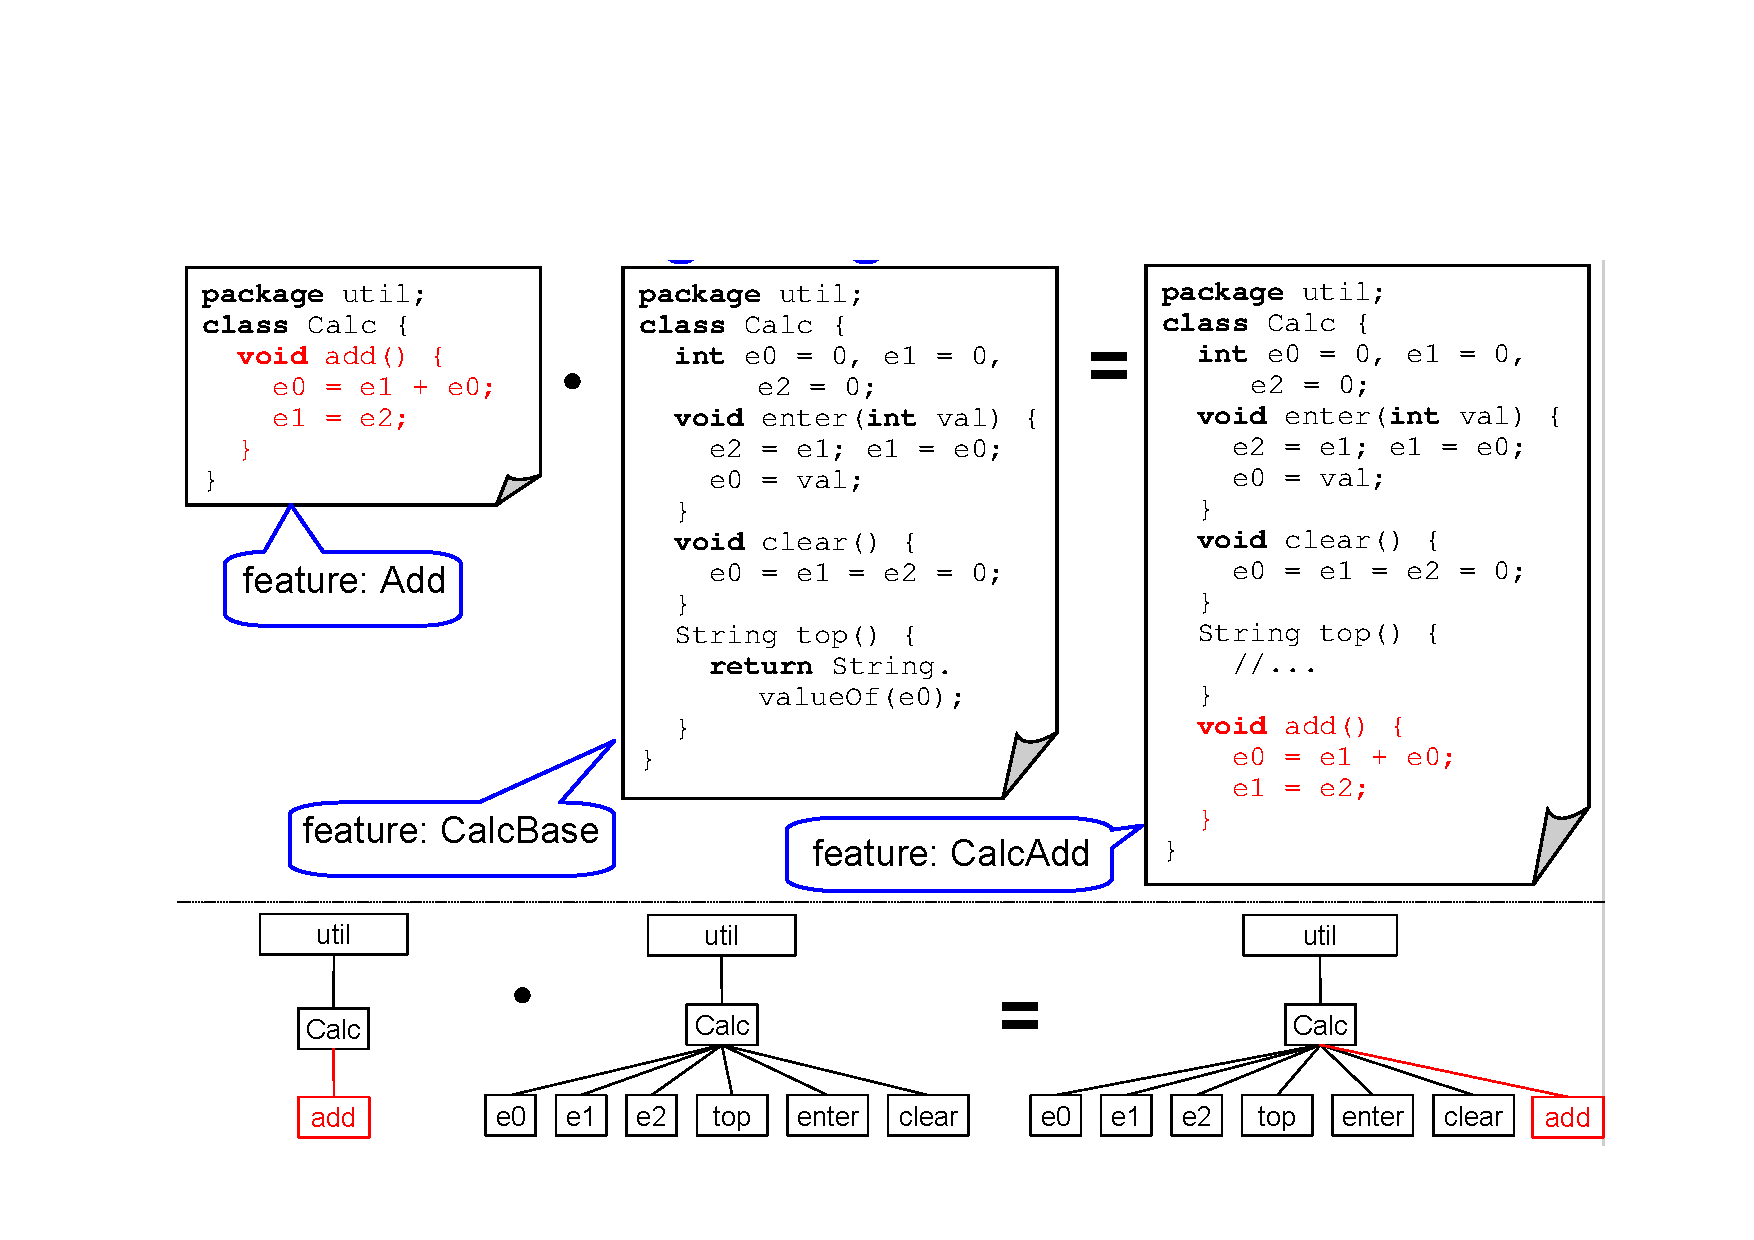
\includegraphics[width=\textwidth]{FOPexample}\\
		\tiny\url{http://wwwiti.cs.uni-magdeburg.de/iti_db/lehre/epmd/2009/slides/06_FOP.pdf}
	\end{center}
\end{frame}

\subsection{Configuration}
\begin{frame}%[fragile]
	\frametitle{\insertsubsection}
	\begin{center}
		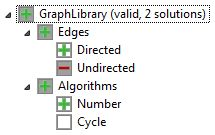
\includegraphics[scale=.75]{conf}
	\end{center}
	\begin{itemize}
		\item Selection of features
		\item Composition of features results in a program variant
		\item Not all combinations are useful
	\end{itemize}
\end{frame}

\subsection{Feature Model}
\begin{frame}%[fragile]
	\frametitle{\insertsubsection}
	\begin{itemize}
		\item Specifies valid combinations of features
		\item Graphically represented by a feature diagram
		\item Created for a particular domain
		\item Describes a software product line (SPL)
	\end{itemize}
	\begin{center}
    \begin{tikzpicture}
      \node at (0,0) {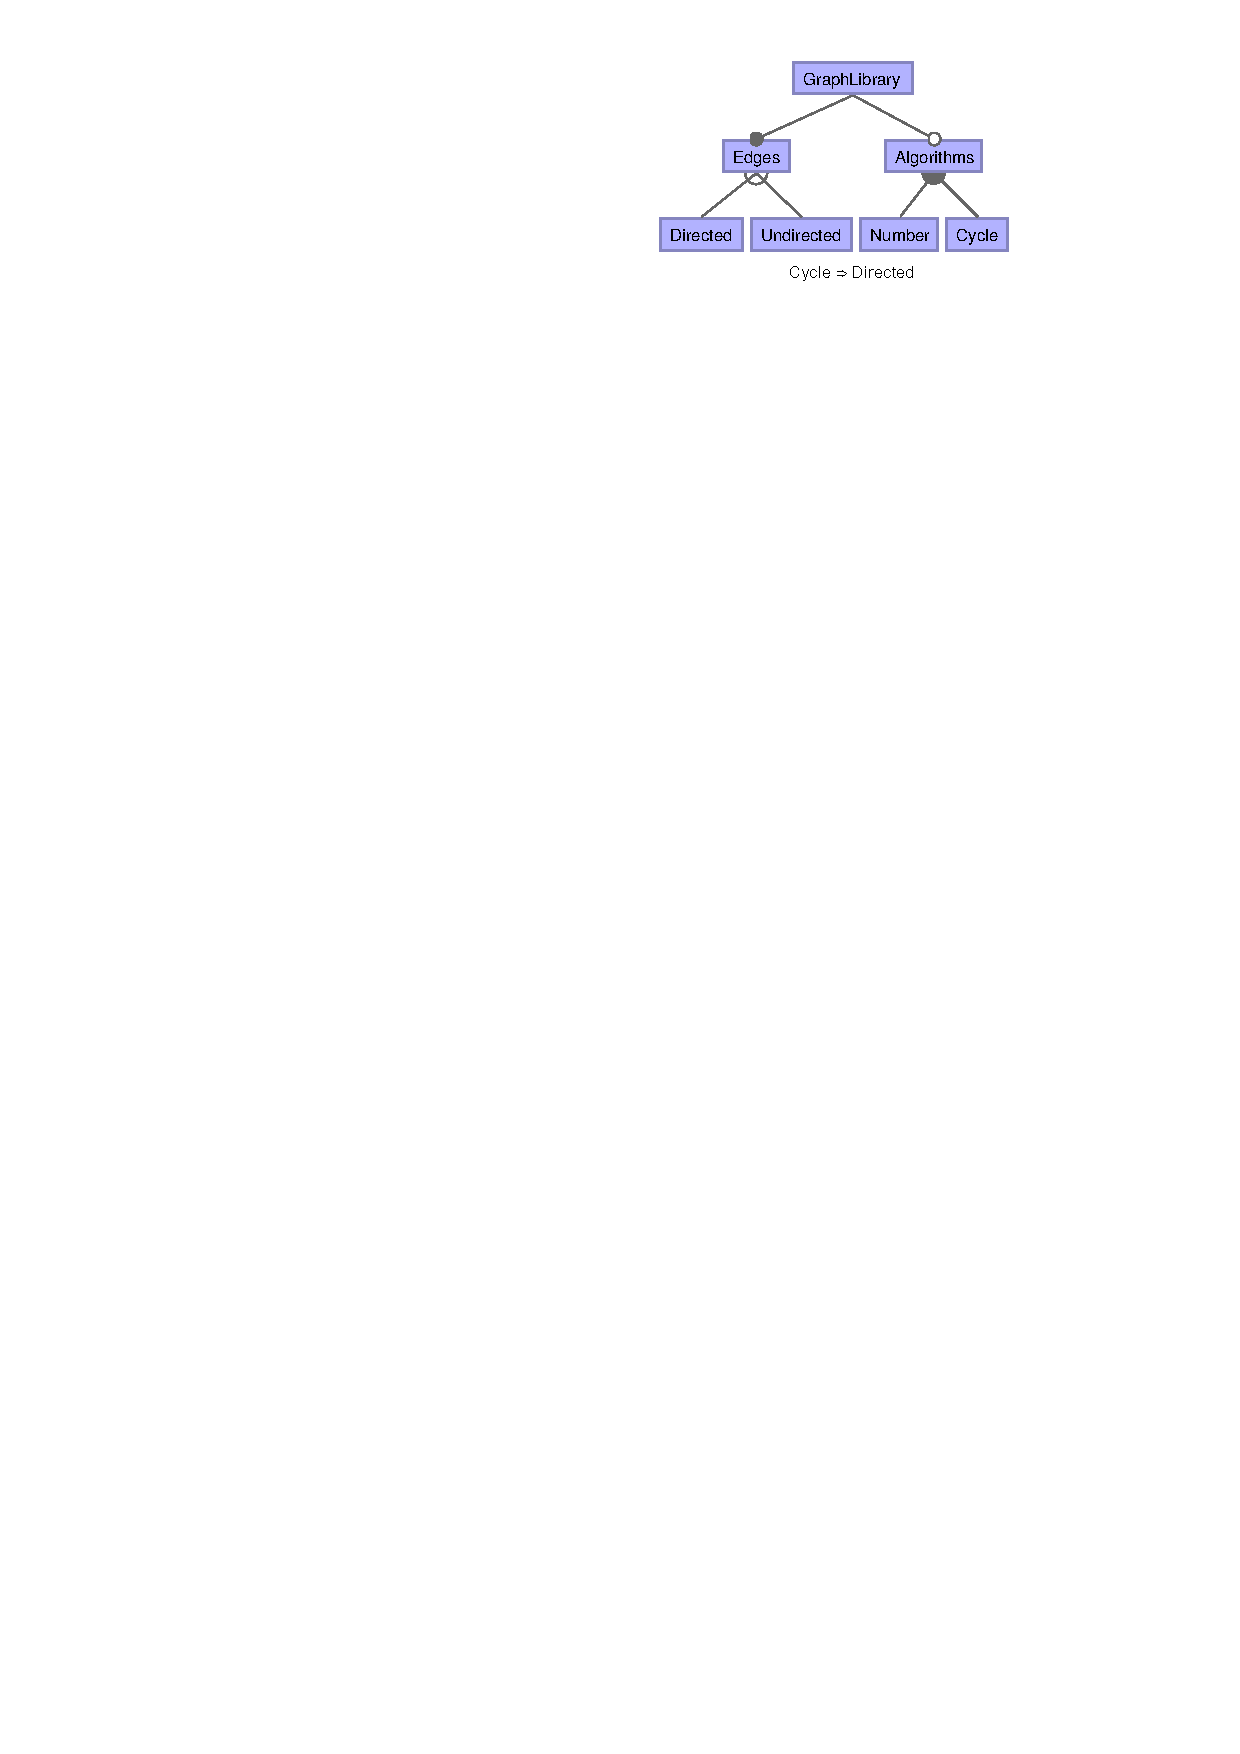
\includegraphics[scale=0.75]{tinygpl1}};
      \node[overlay,inner sep=.5mm,shape=rectangle,draw] at (4.5,-0.9) {
				\begin{minipage}{21mm}
					\tiny
					\begin{flushleft}
						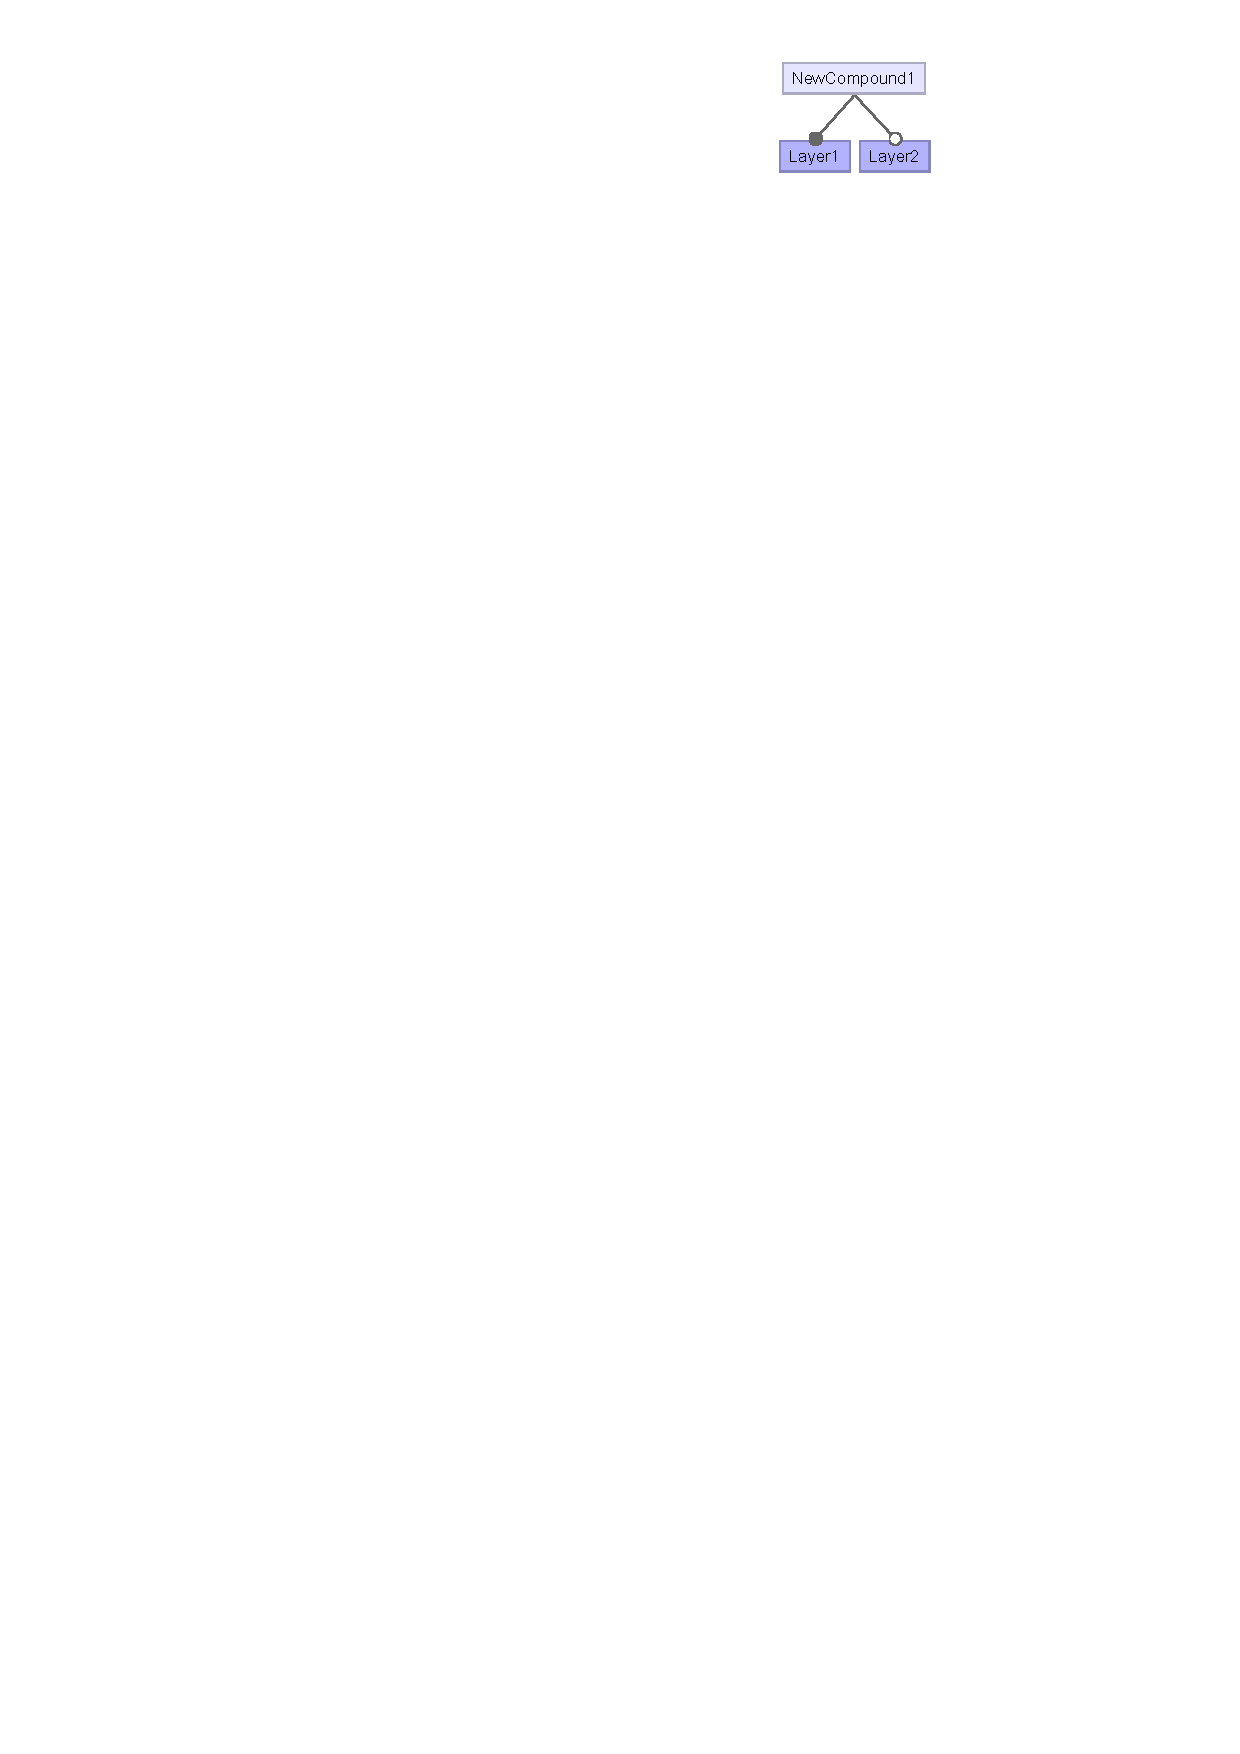
\includegraphics[trim=12.5mm 10mm 14mm 5.5mm,clip,scale=0.6]{fm_and}\ And-group\\[.5mm]
						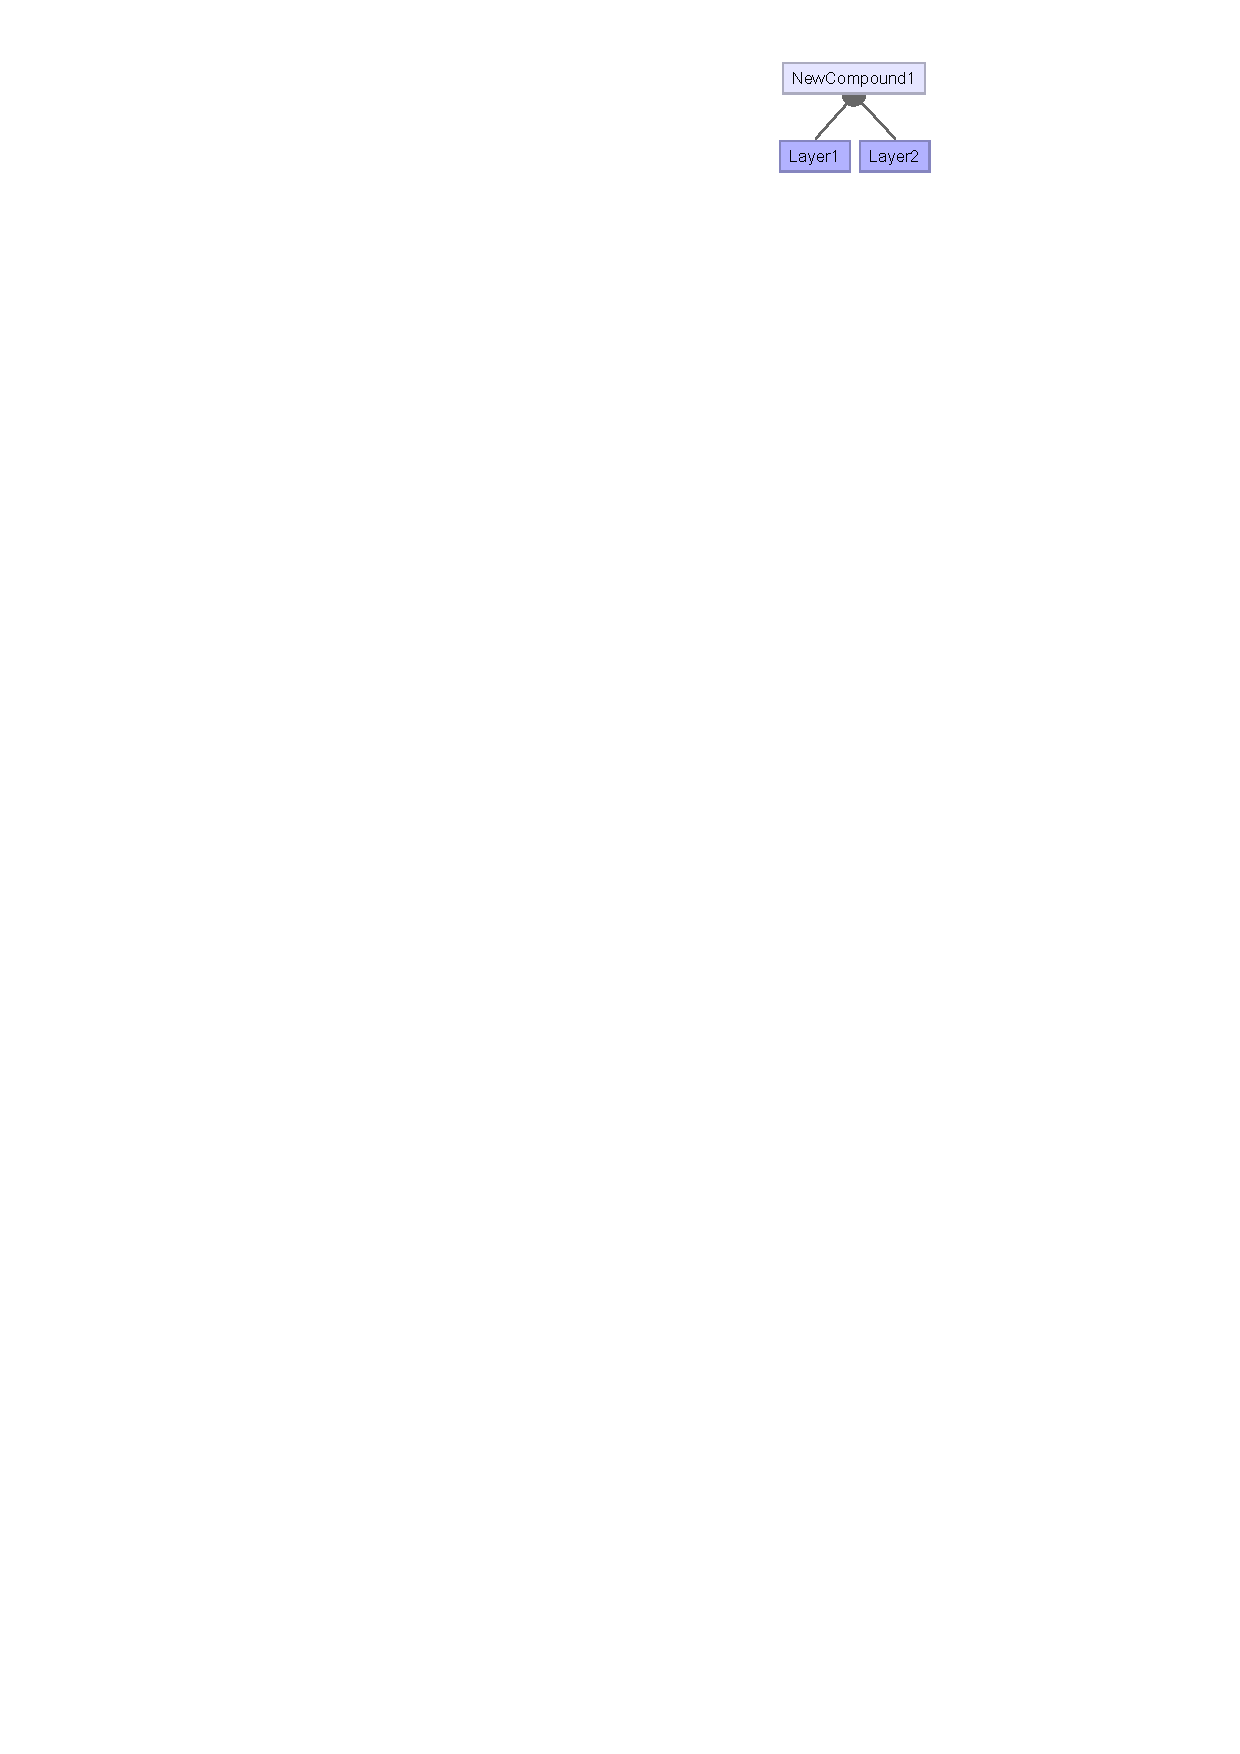
\includegraphics[trim=12.5mm 10mm 14mm 5.5mm,clip,scale=0.6]{fm_or}\ Or-group\\[.5mm]
						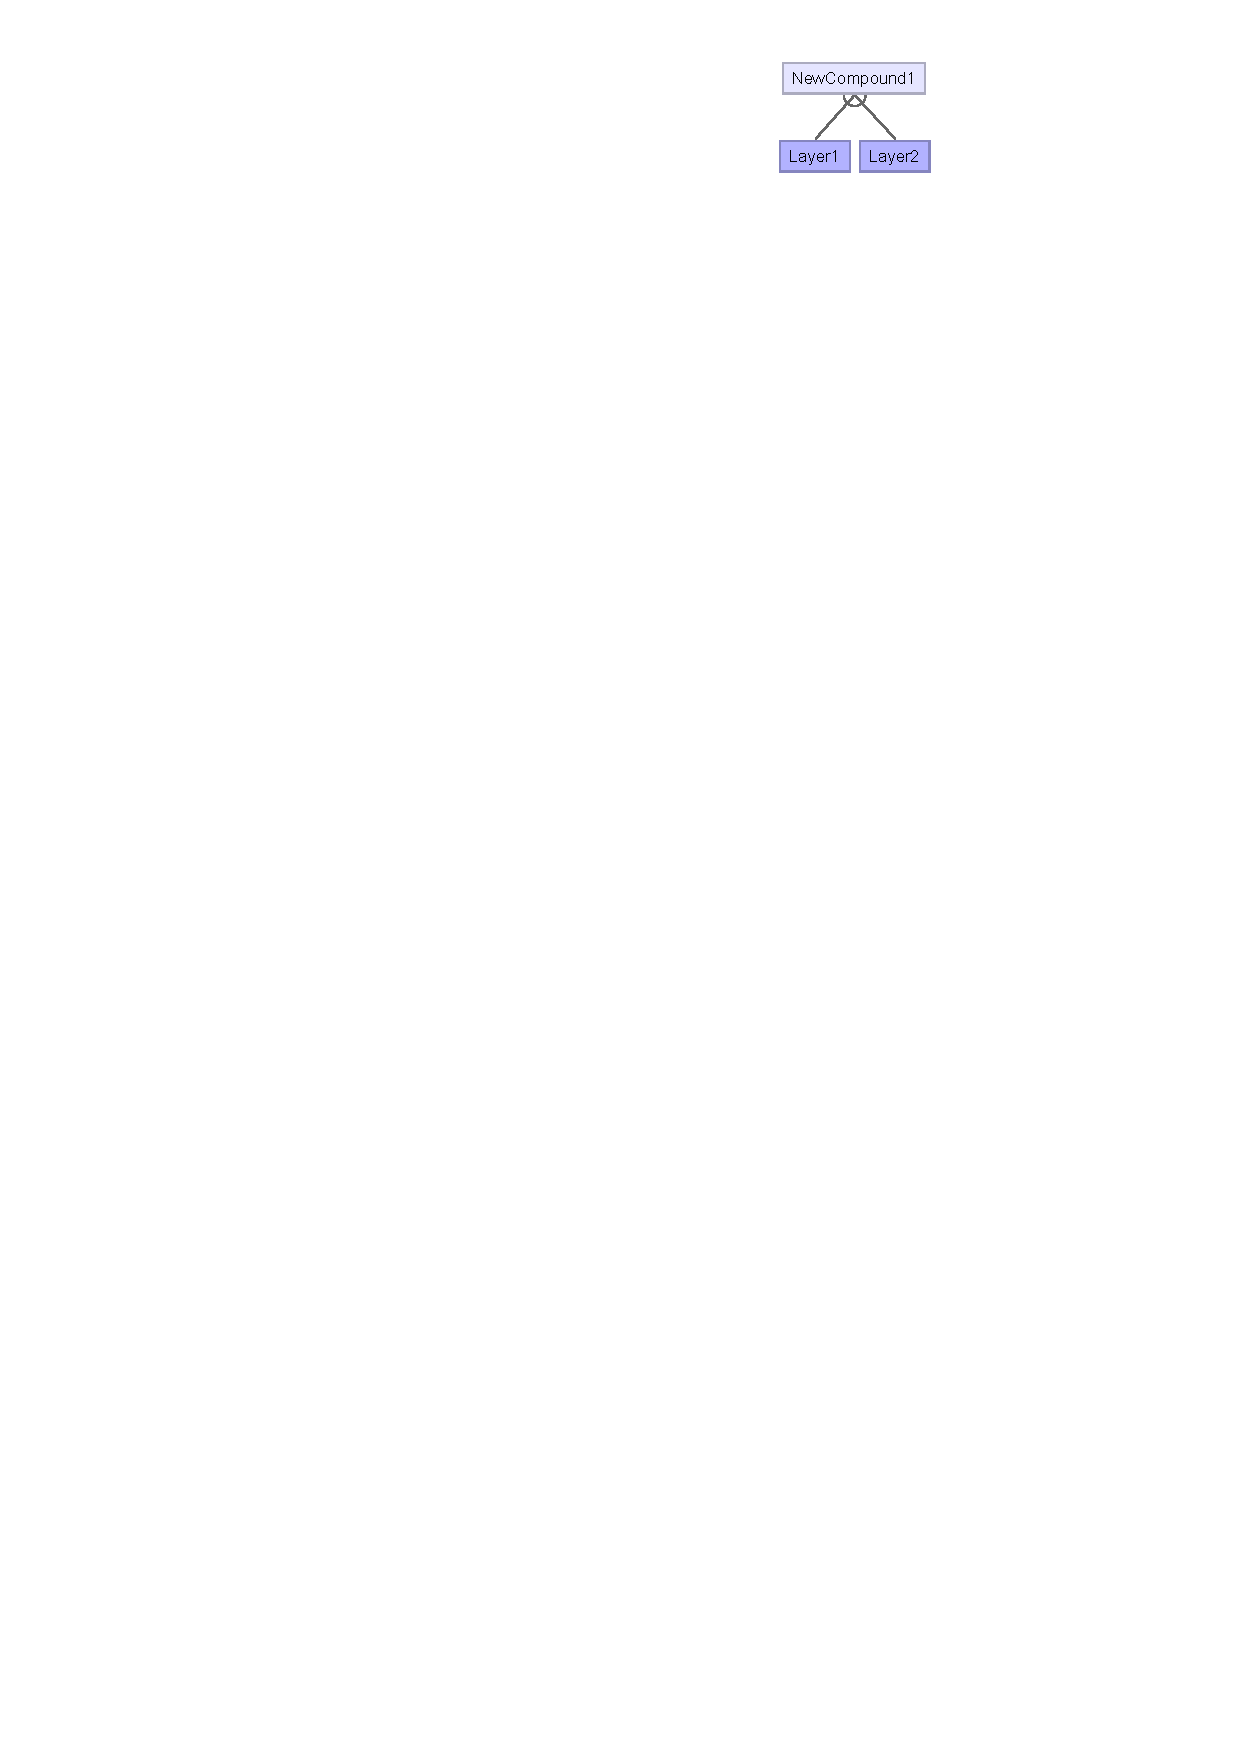
\includegraphics[trim=12.5mm 10mm 14mm 5.5mm,clip,scale=0.6]{fm_alt}\ Alternative-group\\[.5mm]
						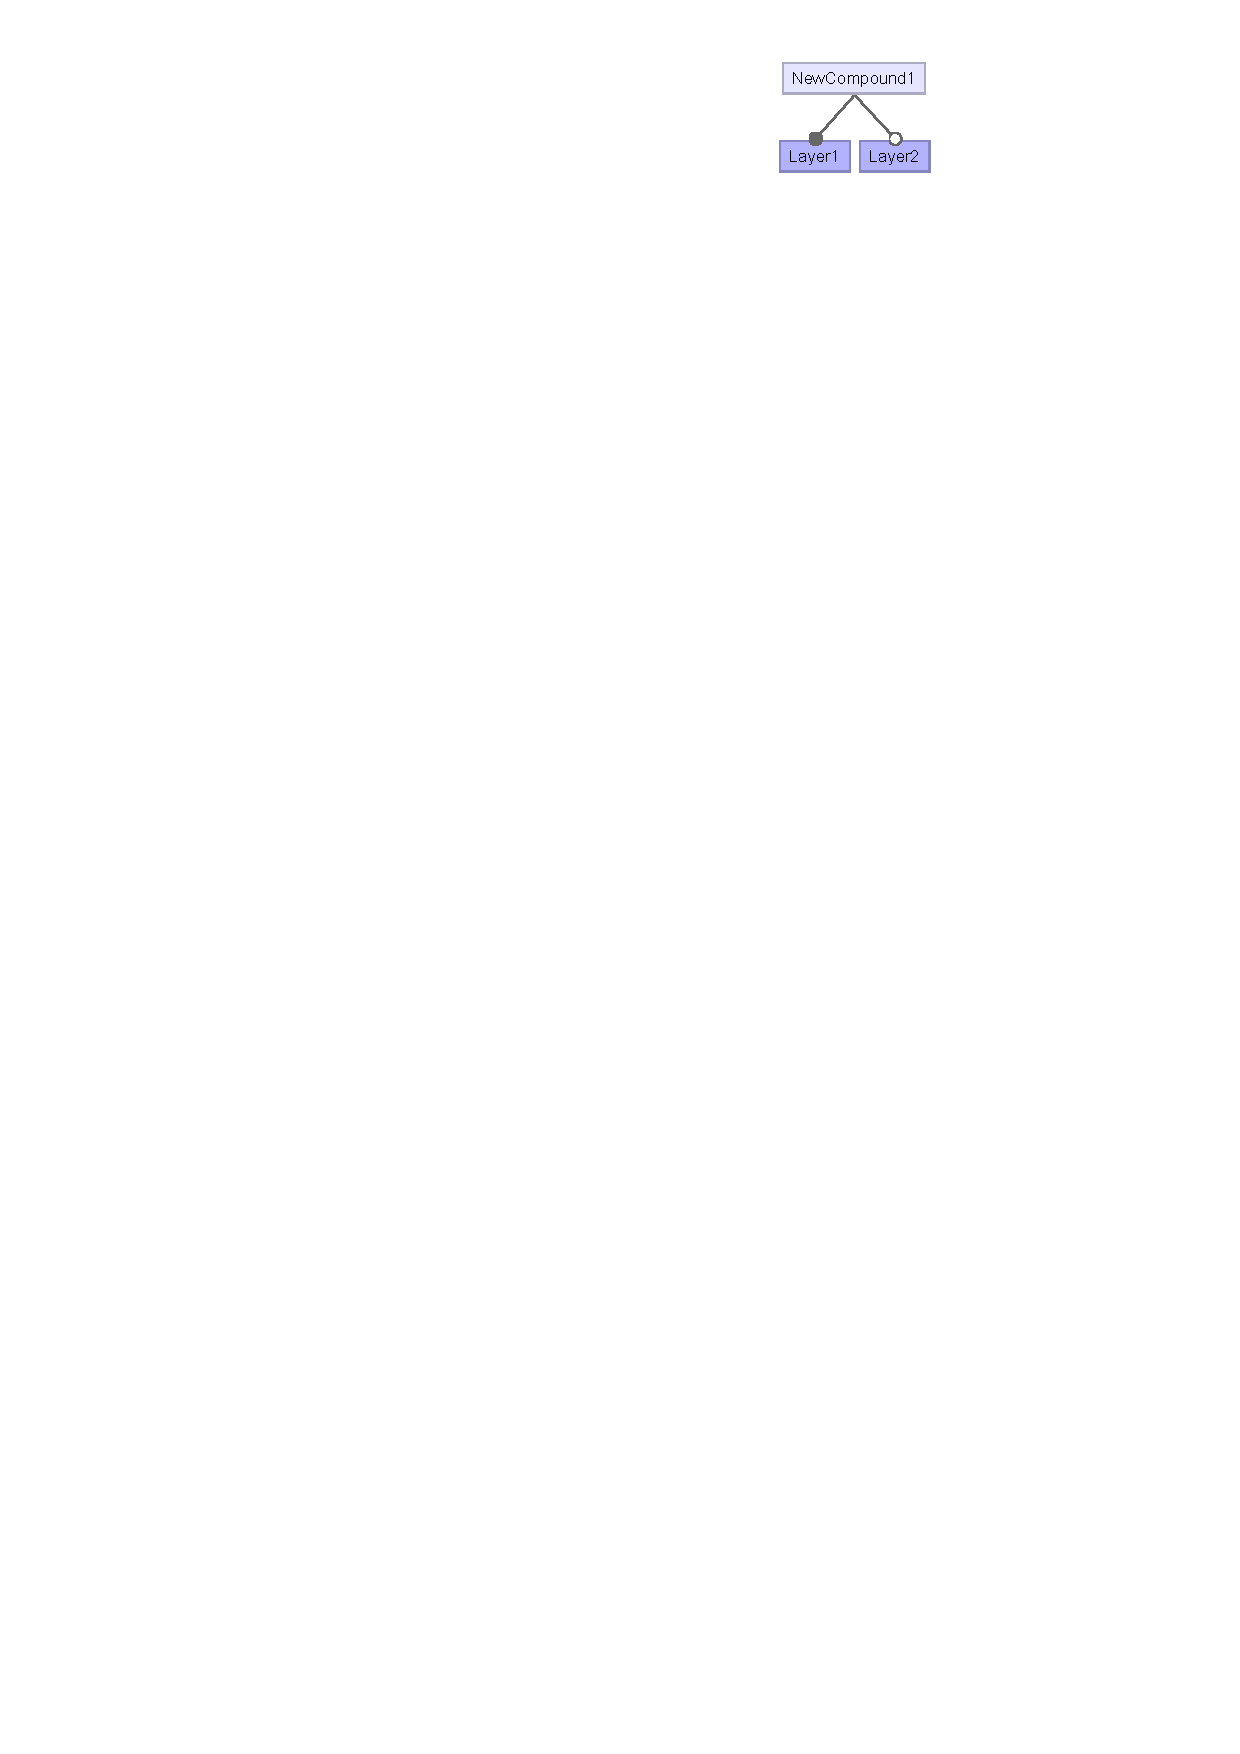
\includegraphics[trim=6mm 4.5mm 21mm 11mm,clip,scale=0.6]{fm_and}\ Mandatory\\[.5mm]
						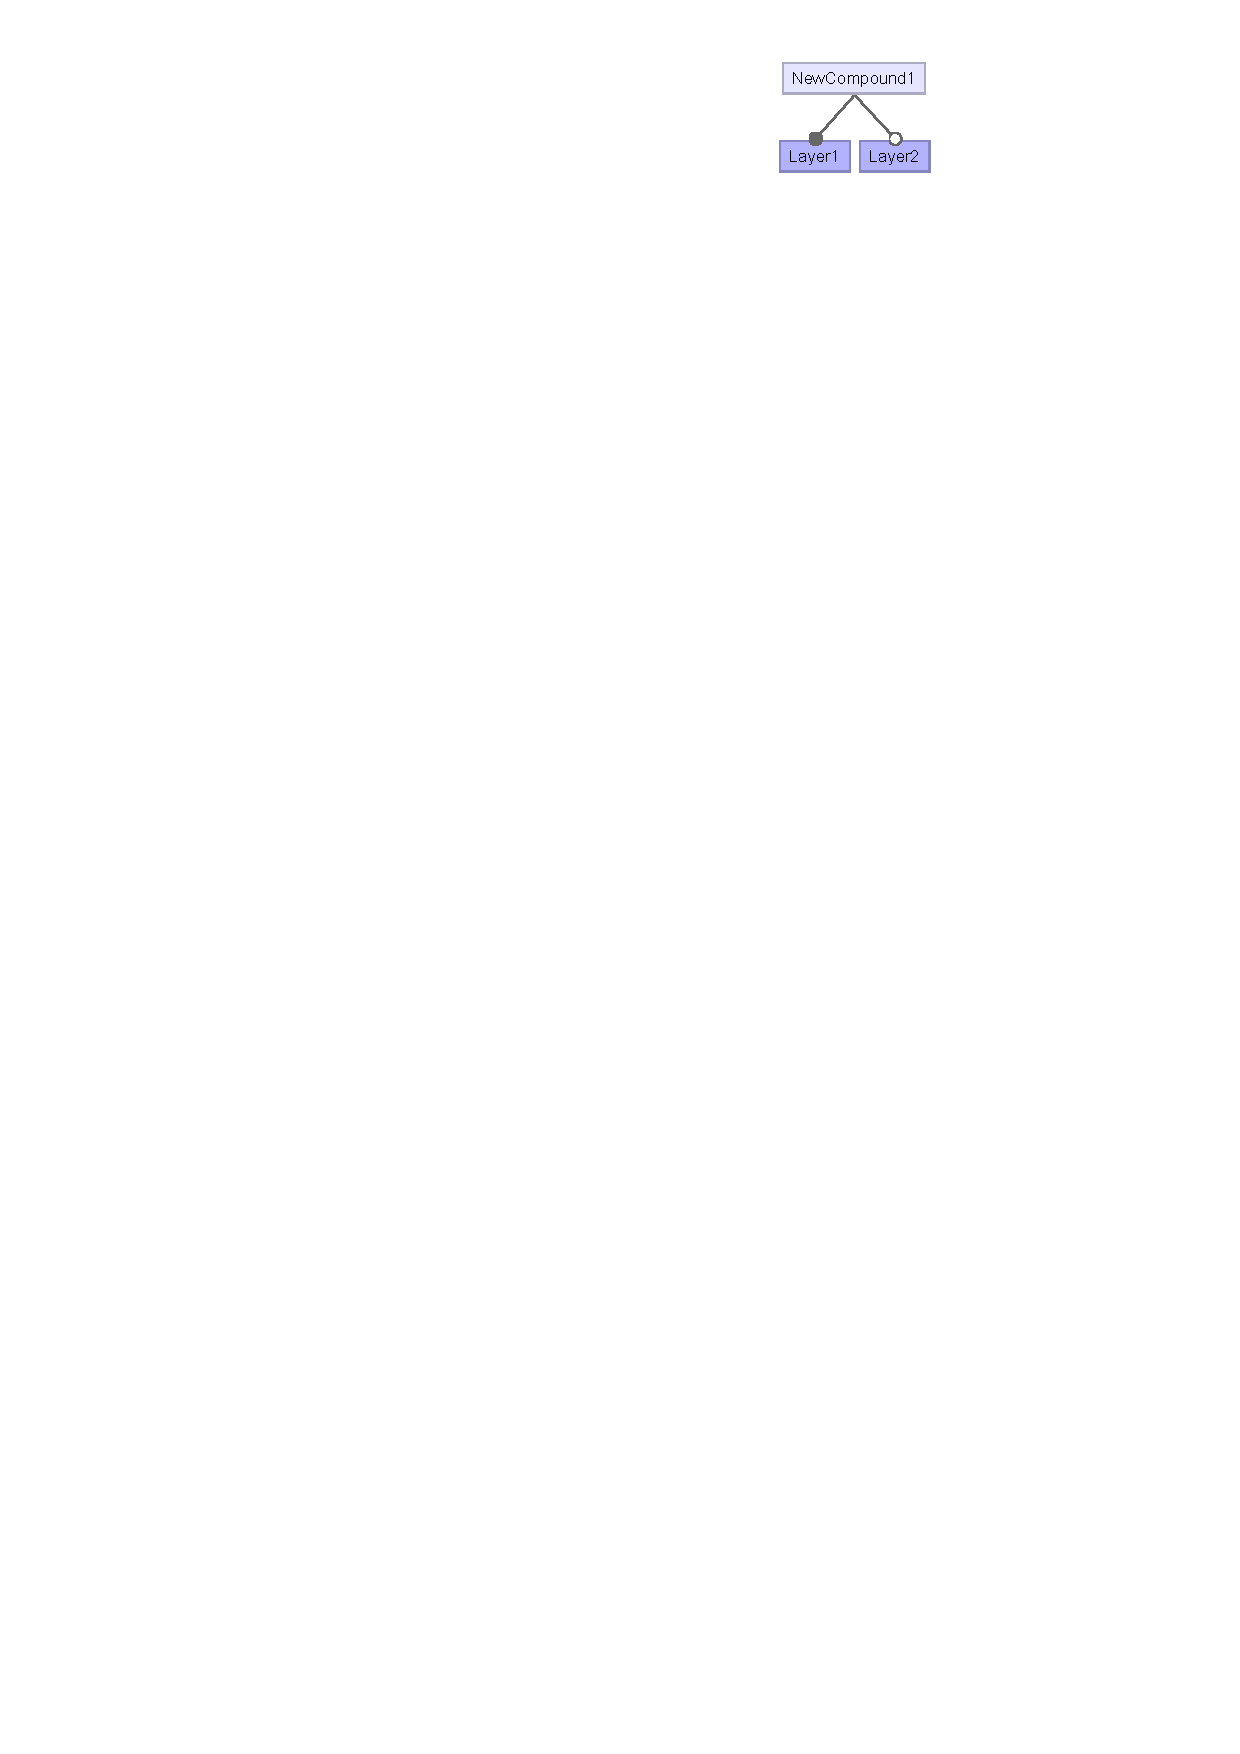
\includegraphics[trim=19.5mm 4.5mm 7.5mm 11mm,clip,scale=0.6]{fm_and}\ Optional
					\end{flushleft}
				\end{minipage}
			};
      \uncover<2>{
	      \node[overlay] (label) at (-2.0,1.2) {\color{red}\footnotesize And-group};
	      \draw[red,thick,-latex,overlay] (label) -- (-0.2,0.8);
			}      
      \uncover<3>{
	      \node[overlay] (label) at (-2.9,0.6) {\color{red}\footnotesize Mandatory};
	      \draw[red,thick,-latex,overlay] (label) -- (-1.1,0.45);
			}      
      \uncover<4>{
	      \node[overlay] (label) at (2.9,1.0) {\color{red}\footnotesize Optional};
	      \draw[red,thick,-latex,overlay] (label) -- (1.4,0.45);
			}      
      \uncover<5>{
	      \node[overlay] (label) at (-3.4,-0.4) {\color{red}\footnotesize Alternative-group};
	      \draw[red,thick,-latex,overlay] (label) -- (-1.2,-0.1);
			}      
      \uncover<6>{
	      \node[overlay] (label) at (3,0.1) {\color{red}\footnotesize Or-group};
	      \draw[red,thick,-latex,overlay] (label) -- (1.4,-0.1);
			}      
      \uncover<7>{
	      \node[overlay] (label) at (-3.1,-1.4) {\color{red}\footnotesize Cross-tree constraints};
	      \draw[red,thick,-latex,overlay] (label) -- (-0.6,-1.3);
			}
			\only<8>{}
    \end{tikzpicture}
	\end{center}
\end{frame}

\subsection{Composition Engines}
\begin{frame}%[fragile]
	\frametitle{\insertsubsection}
	Command-line tools used to compose files within FeatureIDE:\\[5mm]
	\begin{itemize}
		\item AHEAD (jampack): .jak (Java 1.4)\\
		  \url{http://userweb.cs.utexas.edu/~schwartz/ATS.html}\\[5mm]
		\item FeatureC++: .cpp (C++)\\
		  \url{http://www.fosd.de/fcpp}\\[5mm]
		\item FeatureHouse: .java (Java 1.5), .cs (C\#), .c/.h (C), .hs (Haskell), .jj (JavaCC), .als (Alloy), .xmi (UML)\\
		  \url{http://www.fosd.de/fh}		
	\end{itemize}
\end{frame}

\newcommand{\picfontsize}{\footnotesize}
\newcommand{\picfm}{\picfontsize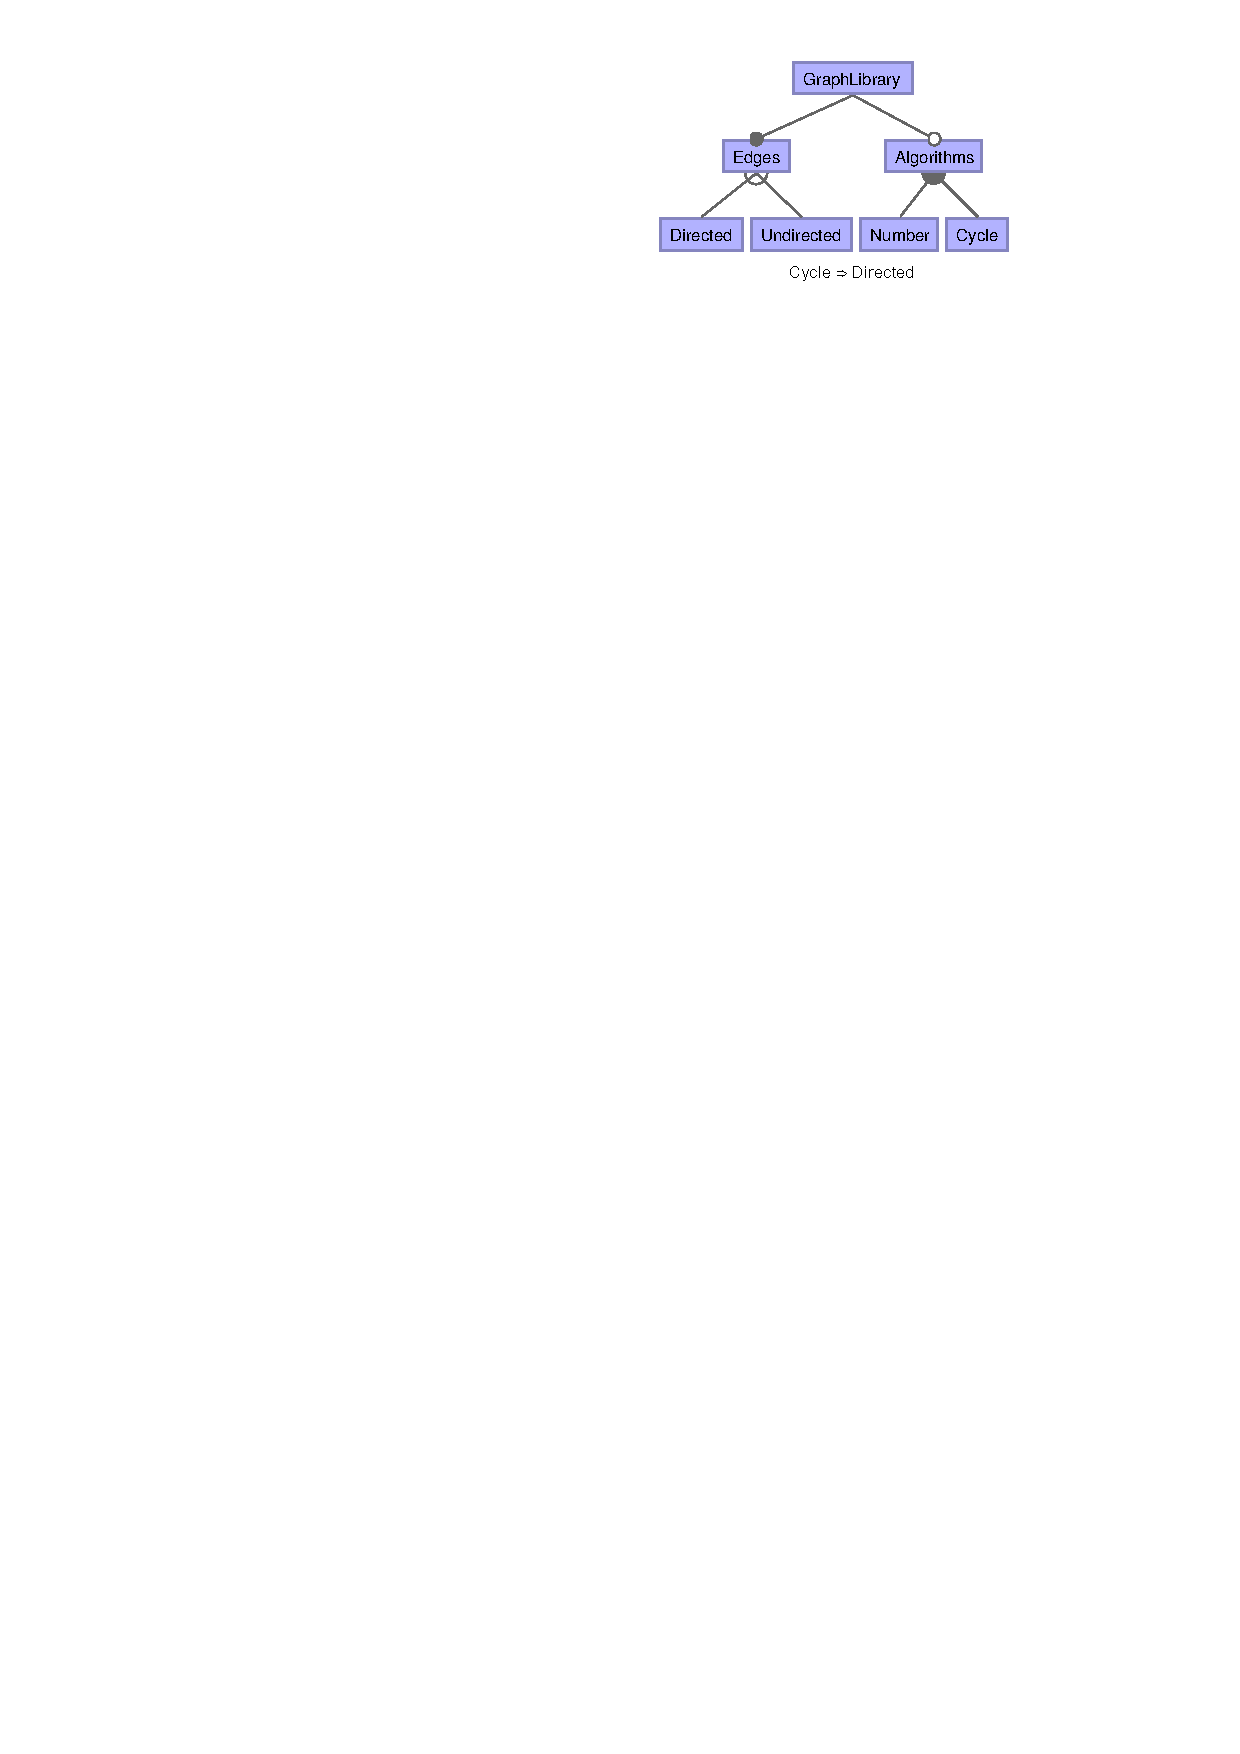
\includegraphics[width=.8\textwidth]{tinygpl1}\\Feature Model}
\newcommand{\piccodebase}{\picfontsize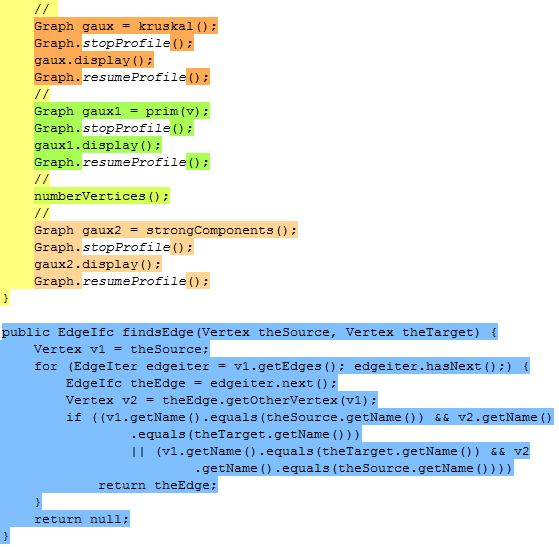
\includegraphics[width=.5\textwidth]{codebase1}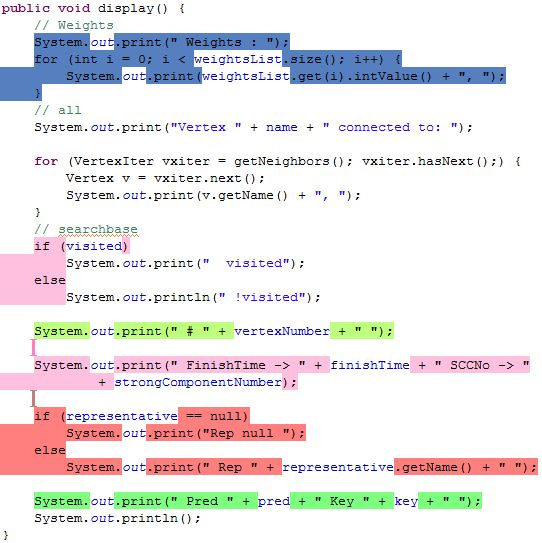
\includegraphics[width=.5\textwidth]{codebase2}\\Feature Modules}
\newcommand{\picconf}{\picfontsize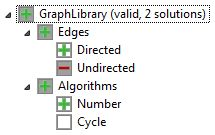
\includegraphics[width=.85\textwidth]{conf}\\Configurations}
\newcommand{\picgen}{\picfontsize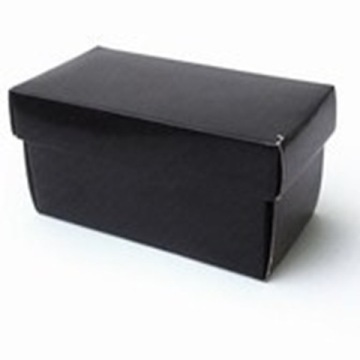
\includegraphics[width=.5\textwidth]{blackbox}\\Composer}
\newcommand{\picvariant}{\picfontsize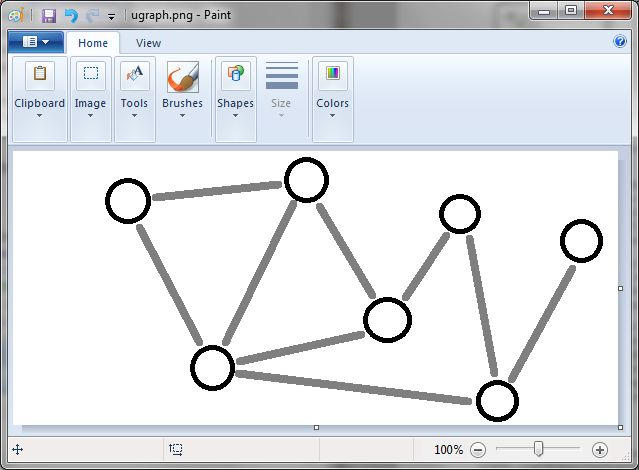
\includegraphics[width=.75\textwidth]{programvariant}\\Program Variants}
\newcommand{\mnode}[3]{
	\node[xshift=.3em, yshift=.3em, #1] (#2x) {};
	\node[#1] {};
	\node[xshift=-.3em, yshift=-.3em, #1] (#2) {#3}
}
\subsection{Feature-Oriented Software Development}
\begin{frame}%[fragile]
	\frametitle{\insertsubsection}
	\begin{center}
		\begin{tikzpicture}[node distance=8mm]
			\node[node1s] (fm) {\picfm};
			\node[node1s, right=of fm]	(codebase) {\piccodebase};
			\mnode{node1s, below=of fm}{configuration}{\picconf};
			\node[node1s, below=of codebase] (generator) {\picgen};
			\mnode{node1s, right=of generator}{variants}{\picvariant};
			\draw[edge2] (fm) -- (configurationx);
			%\draw[edge2] (fm) -- (codebase);
			\draw[edge1] (configurationx) -- (generator);
			\draw[edge1] (codebase) -- (generator);
			\draw[edge1] (generator) -- (variants);
		\end{tikzpicture}
	\end{center}
\end{frame}

\begin{frame}%[fragile]
	\frametitle{Content}
	\begin{itemize}
		\item {\color{grayed}What is Feature-Oriented Software Development?}\\[5mm]
		\item What functionality does FeatureIDE provide?
			\begin{itemize}
				\item Feature Model Editor + Edit View
				\item Configuration Editor
				\item Jak Editor
				\item Collaboration Diagram
				\item Feature Project Builder
				\item Run Configurations
				\item Creation Wizards\\[5mm]
			\end{itemize}
		\item {\color{grayed}How to start working with FeatureIDE?}
	\end{itemize}
\end{frame}

\section{Functionality of FeatureIDE}

\subsection{Feature Model Editor: Feature Diagram}
\begin{frame}%[fragile]
	\frametitle{\insertsubsection}
	\begin{itemize}
		\item<1-> Double click to change connections and mandatory property
		\item<2-> Single click to rename features
		\item<3-> Right click to open context menu for features/connections
		\item<4-> Drag \uncover<5->{and drop features}
		\item<6-> Context menu \uncover<7->{to open Constraint Editor}
	\end{itemize}
	\begin{center}
		\only<1>{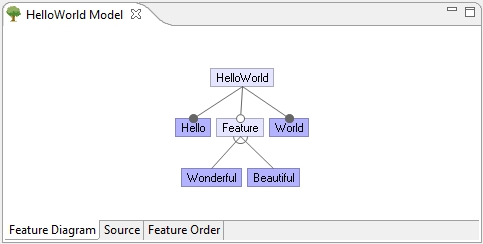
\includegraphics[scale=.5]{hw_fme_fd}}
		\only<2>{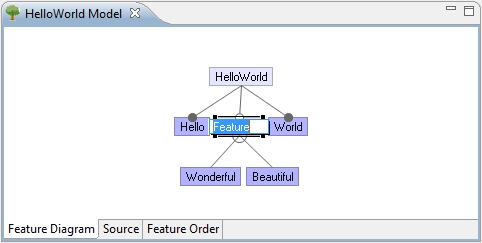
\includegraphics[scale=.5]{hw_fme_fd_rename}}
		\only<3>{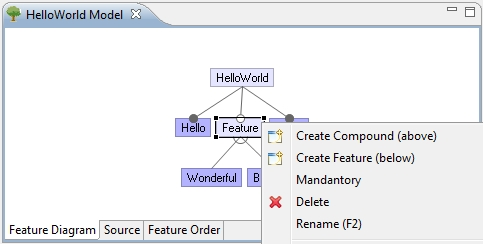
\includegraphics[scale=.5]{hw_fme_fd_menu}}
		\only<4>{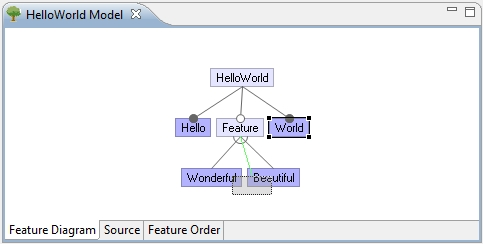
\includegraphics[scale=.5]{hw_fme_fd_drag}}
		\only<5>{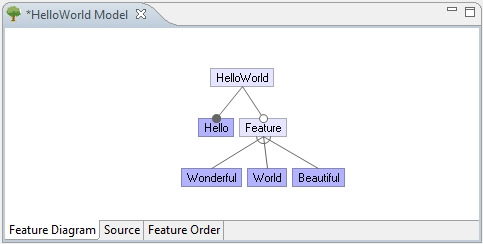
\includegraphics[scale=.5]{hw_fme_fd_drop}}
		\only<6>{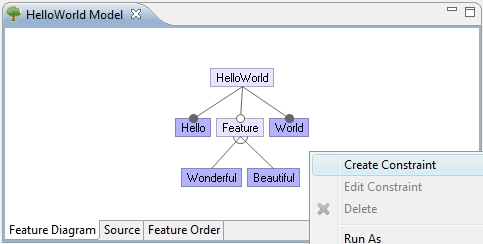
\includegraphics[scale=.5]{hw_fme_fd_menu2}}
		\only<7>{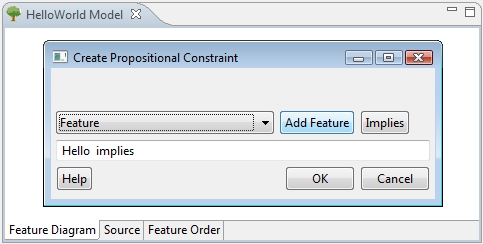
\includegraphics[scale=.5]{hw_fme_fd_ce}}
	\end{center}
\end{frame}

\subsection{Feature Model Editor - Grammar}
\begin{frame}[fragile]
	\frametitle{\insertsubsection}
	\begin{itemize}
		\item Source tab contains the GUIDSL grammar representation
		\item \verb![]! - optional feature
		\item \verb!|! - Or-group -or- Alternative-group depending on parent
		\item \verb!+! - mandatory feature and Or-group below
		\item \verb!*! - optional feature and Or-group below
	\end{itemize}
	\begin{center}
		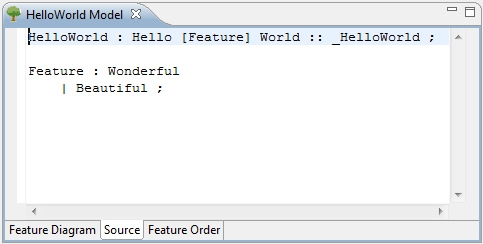
\includegraphics[scale=.5]{hw_fme_src}
	\end{center}
\end{frame}

\subsection{Feature Model Editor - Feature Order}
\begin{frame}%[fragile]
	\frametitle{\insertsubsection}
	\begin{itemize}
		\item Order of features matters: can influence program behavior
		\item Default order: pre-order traversal of the feature diagram
		\item User-defined order possible
		\item Applies to all configurations
	\end{itemize}
	\begin{center}
		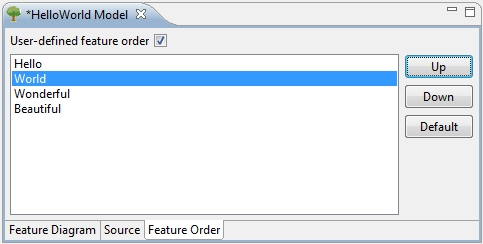
\includegraphics[scale=.5]{hw_fme_order}
	\end{center}
\end{frame}

\subsection{Feature Model Editor - Synchronization}
\begin{frame}%[fragile]
	\frametitle{\insertsubsection}
	Before saving:
	\begin{itemize}
		\item When switching tab, changes are propagated\\[5mm]
	\end{itemize}
	When saving:
	\begin{itemize}
		\item Feature folders are created, removed, and renamed
		\item Updating order of features in configurations
		\item Checking which configurations are valid/invalid
		\item Current content of Configuration Editor updated
	\end{itemize}
	\begin{center}
		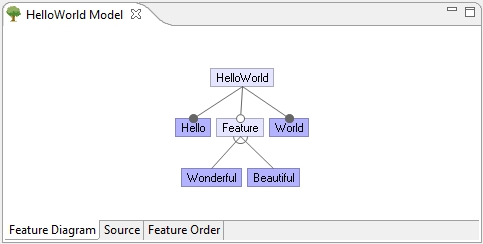
\includegraphics[scale=.2]{hw_fme_fd}~
		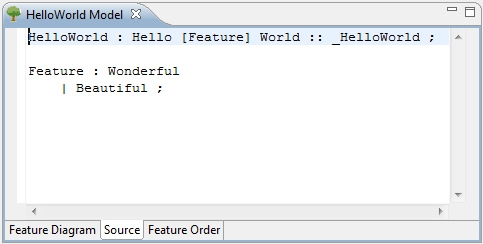
\includegraphics[scale=.2]{hw_fme_src}~
		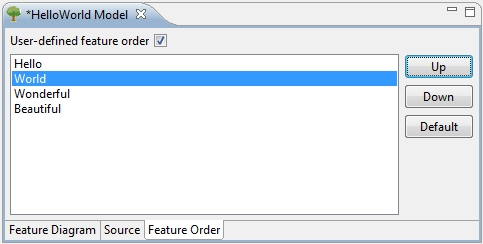
\includegraphics[scale=.2]{hw_fme_order}
	\end{center}
\end{frame}

\subsection{Feature Model Edit View}
\begin{frame}%[fragile]
	\frametitle{\insertsubsection}
	\begin{itemize}
		\item \ldots
		\item \ldots
		\item \ldots
	\end{itemize}
\end{frame}

\subsection{Configuration Editor}
\begin{frame}%[fragile]
	\frametitle{\insertsubsection}
	\begin{itemize}
		\item \ldots
		\item \ldots
		\item \ldots
	\end{itemize}
\end{frame}

\subsection{Jak Editor}
\begin{frame}%[fragile]
	\frametitle{\insertsubsection}
	\begin{itemize}
		\item \ldots
		\item \ldots
		\item \ldots
	\end{itemize}
\end{frame}

\subsection{Collaboration Diagram}
\begin{frame}%[fragile]
	\frametitle{\insertsubsection}
	\begin{itemize}
		\item \ldots
		\item \ldots
		\item \ldots
	\end{itemize}
\end{frame}

\subsection{Feature Project Builder}
\begin{frame}%[fragile]
	\frametitle{\insertsubsection}
	\begin{itemize}
		\item \ldots
		\item \ldots
		\item \ldots
	\end{itemize}
\end{frame}

\subsection{Run Configurations}
\begin{frame}%[fragile]
	\frametitle{\insertsubsection}
	\begin{itemize}
		\item \ldots
		\item \ldots
		\item \ldots
	\end{itemize}
\end{frame}

\subsection{Creation Wizards}
\begin{frame}%[fragile]
	\frametitle{\insertsubsection}
	\begin{itemize}
		\item \ldots
		\item \ldots
		\item \ldots
	\end{itemize}
\end{frame}

\begin{frame}%[fragile]
	\frametitle{Content}
	\begin{itemize}
		\item {\color{grayed}What is Feature-Oriented Software Development?\\[5mm]
		\item What functionality does FeatureIDE provide?}\\[5mm]
		\item How to start working with FeatureIDE?
		\begin{itemize}
			\item FeatureIDE installation
			\item FeatureIDE project structure
			\item Cheat Sheet
		\end{itemize}
	\end{itemize}
\end{frame}

\section{How to Start}

\subsection{Installation of FeatureIDE}
\begin{frame}%[fragile]
	\frametitle{\insertsubsection}
	\begin{itemize}
		\item \ldots
		\item \ldots
		\item \ldots
	\end{itemize}
\end{frame}

\subsection{FeatureIDE Project Structure}
\begin{frame}%[fragile]
	\frametitle{\insertsubsection}
		\begin{columns}
		\column{.4\textwidth}
			\only<1>{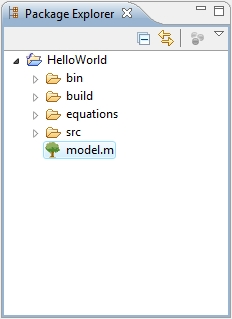
\includegraphics[scale=0.55]{hw_pe_model}}
			\only<2>{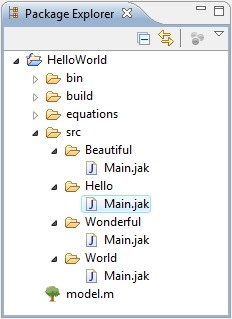
\includegraphics[scale=0.55]{hw_pe_src}}
			\only<3>{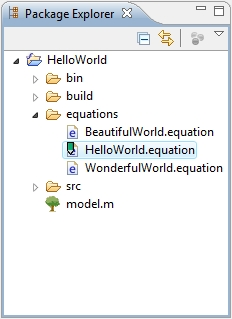
\includegraphics[scale=0.55]{hw_pe_conf}}
			\only<4>{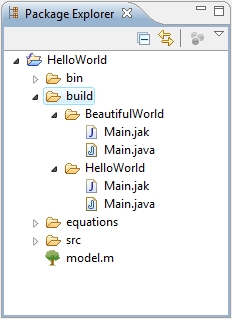
\includegraphics[scale=0.55]{hw_pe_build}}
			\only<5>{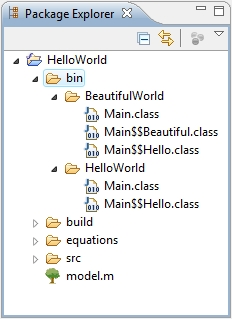
\includegraphics[scale=0.55]{hw_pe_bin}}
		\column{.6\textwidth}
			\begin{itemize}[<+->]
				\item Feature model file in the GUIDSL-format
				\item Source folder containing a folder for every feature including files to compose
				\item Configurations containing selected features from the feature model
				\item Composed source files for several configurations (might be helpful when debugging)
				\item Binary files for several configurations
			\end{itemize}
	\end{columns}
\end{frame}

\subsection{Cheat Sheet}
\begin{frame}%[fragile]
	\frametitle{\insertsubsection}
	\begin{itemize}
		\item \ldots
		\item \ldots
		\item \ldots
	\end{itemize}
\end{frame}

%\subsection{\ldots}
%\begin{frame}%[fragile]
	%\frametitle{\insertsubsection}
	%\begin{itemize}
		%\item \ldots
		%\item \ldots
		%\item \ldots
	%\end{itemize}
%\end{frame}

\end{document}